\chapter{Background}\label{chap:background}
explain all the things.

global/local citation (for local especially explain harvesting citation contexts and comparing aggregrates to input)

citation marker

four types of numbers (citing/cited documents, reference items citation context)

reference resolution

\begin{figure}
  \centering
    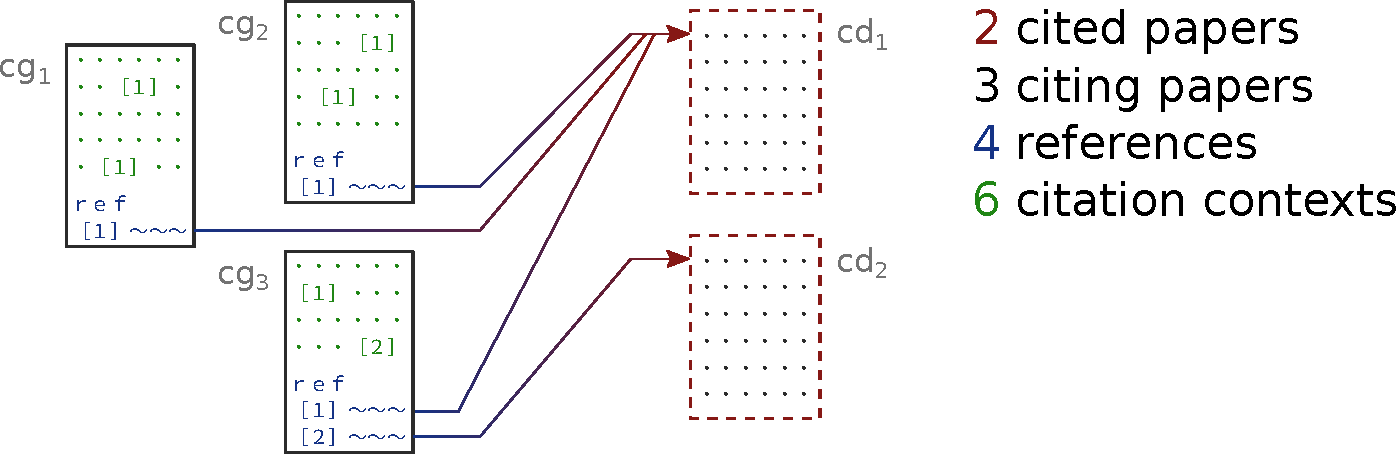
\includegraphics[width=\textwidth]{figures/background/four_types_of_numbers_vertsqueeze.pdf}
  \caption[Four types of numbers.]{Four types of numbers. A toy example with citation pairs $cg_1\rightarrow cd_1$, $cg_2\rightarrow cd_1$, $cg_3\rightarrow cd_1$, $cg_3\rightarrow cd_2$ resulting in 2 cited papers, 3 citing papers, 4 references and 6 citation contexts.}
  \label{fig:fournumbers}
\end{figure}

Algorithm~\ref{alg:nprep}

\begin{algorithm}[ht]
\caption{Construction of $R_{\text{NP}}(c)$}
\label{alg:nprep}
\begin{algorithmic}
    \State $NPs \gets array()$     \alignedComment{empty array}
    \State $w_c \gets tokenize(c)$     \alignedComment{$c$ as an array of words}
    \State $l \gets len(w_c)$       \alignedComment{length of NP to search}
    \While{$l > 0$}
        \State $shift \gets 0$
        \While{$m+shift \leq len(w_c)$}
            \State $slice \gets w_c[shift:(shift+l)]$       \alignedComment{$l$ size slice of $w_c$}
            \If{foo}
                \State bar
            \EndIf
        \EndWhile
        \State $l \gets l-1$
    \EndWhile
\end{algorithmic}
\end{algorithm}
